Suppose we have
%\begin{multicols}{2}
\begin{itemize}
	\item binary columns $\bit{1}$, $\bit{2}$, $\bit{3}$, $\bit{4}$,
	\item counter constant columns \source{}, \target{} and $\target{}\new$,
	\item byte columns \source{}\byte{} and \target{}\byte{},
	\item counter constant columns \source{}\mark{} and \target{}\mark{},
	\item a counter constant column \size{},
	\item ``accumulator'' columns \acc{1}, \acc{2},
	\item a ``powers'' column $\col{P}$,
	\item a ``counter column'' \ct{}.
		%\item[\vspace{\fill}]
\end{itemize}
%\end{multicols}
The interpretation is as follows: 
\source{} and \target{} are counter-constant columns containing limbs viewed respectively as a ``source'' and a ``target'' limb;
\source{}\byte{} and \target{}\byte{} are their respective byte decomposition;
$\target{}\new$ contains the ``new'' value of \target{};
\source{}\mark{} and \target{}\mark{} are markers $\in\{0,1,\dots,\llargeMO\}$ for for \source{} and \target{} respectively;
we expect both
$\col{SM} + (\size{}-1)\leq \llargeMO$ and
$\col{TM} + (\size{}-1)\leq \llargeMO$;
\col{P} is pegged to $\bit{2}$ and computes the appropriate power of $256$ so that we may replace a chunk from $\target$ with a chunk from $\source{}$.
Compare with figure~\ref{fig: one partial to one}.


We collect the following constraints under a collective name
\begin{enumerate}
	\item binary-plateau-constraints:
		\begin{enumerate}
			\item $\plateau(\bit{1}, \target{}\mark{}; \ct{})$
			\item $\plateau(\bit{2}, \target{}\mark{} + \size{}; \ct{})$
			\item $\plateau(\bit{3}, \source{}\mark{}; \ct{})$
			\item $\plateau(\bit{4}, \source{}\mark{} + \size{}; \ct{})$
		\end{enumerate}
	\item chunk-constraints
		\begin{enumerate}
			\item $\compChunk(\acc{1}, \target{}\byte{}, \bit{1}, \bit{2}; \ct{})$ % i.e. $\acc{1}\implies \alpha$
			\item $\compChunk(\acc{2}, \source{}\byte{}, \bit{3}, \bit{4}; \ct{})$ % i.e. $\acc{2}\implies \gamma$
		\end{enumerate}
	\item power-constraint: $\power(\col{P},\bit{2}; \ct{})$
	\item update constraint:
		\[
			\If
			\ct_i = \llargeMO~
			\Then
			\target{}\new{}_i
			=
			\target{}_i
			+
			(\acc{2}_i - \acc{1}_i)\cdot\col{P}_i.
		\]
\end{enumerate}
We encapsulate all these constraints under a single relation
\[
	\onePartialToOne
	\left( \begin{array}{c}
		\source{}, \target{}, \target{}\new{};
		\source{}\byte{}, \target{}\byte{};\\
		\acc{1}, \acc{2}; \col{P}; \\
		\source{}\mark{}, \target{}\mark{}; \size{};\\
		\bit{1}, \bit{2}, \bit{3}, \bit{4}; \ct{};
	\end{array} \right)
\]
\begin{figure}[h!]
	\centering
	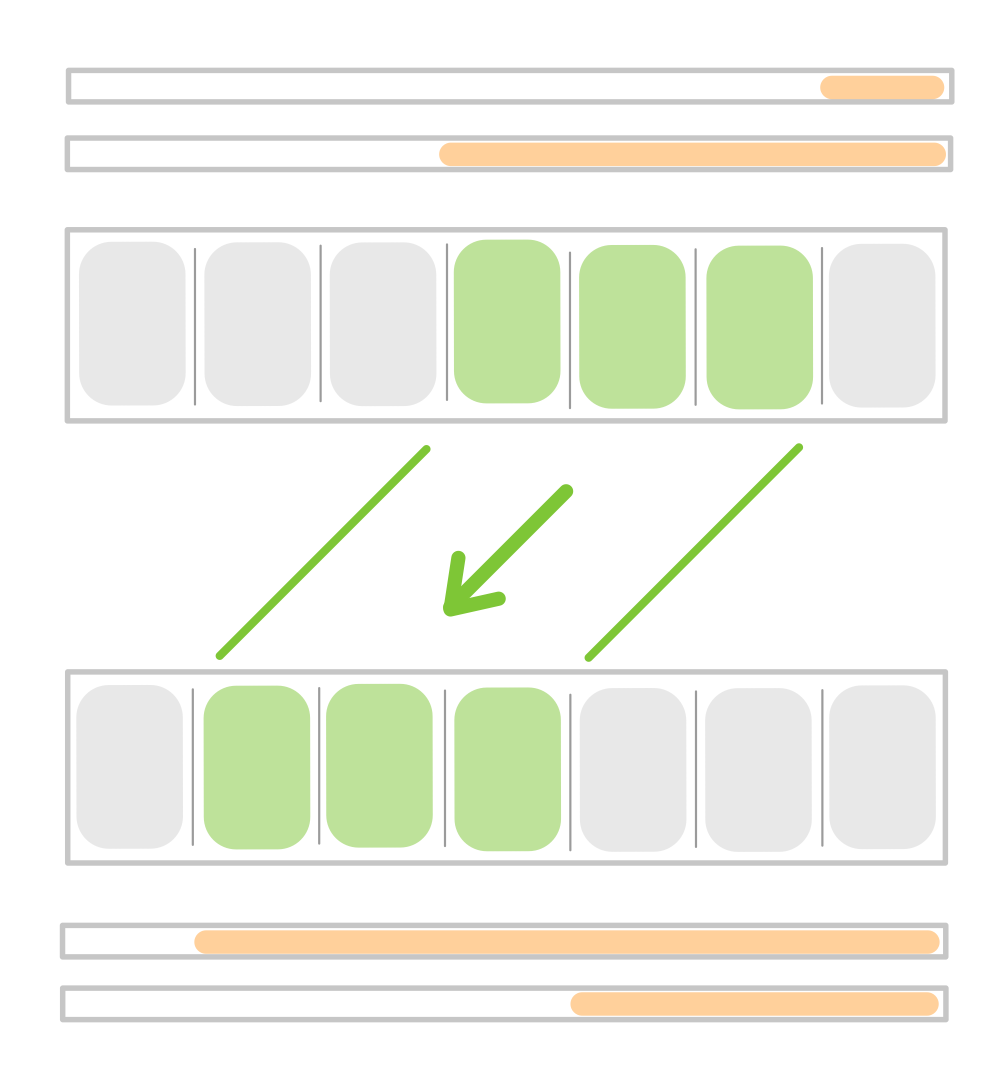
\includegraphics[width = 0.4\textwidth]{drawing/1_partial_to_1}
	\label{fig: one partial to one}
	\caption{Representation of the constraints implemented by $\onePartialToOne$.}
\end{figure}
